%=====================================================================
\section{Weekend 2--4 October: sweep, mirror runs, ellipses, $k$ dependence}\label{sec:weekend}

\subsection{Main sweep: where circles keep the layer}
All 1112 runs of the positive-winding sweep ($\zeta=0.07$, $k=1$--20, $\rho=0.03$--0.50, 3 seeds, plus passive references)
were analysed with the knee of $Q(r)$, the wall Fourier analysis and the site rule (Fig.~\ref{fig:diagram}).
\begin{figure}[h]\centering
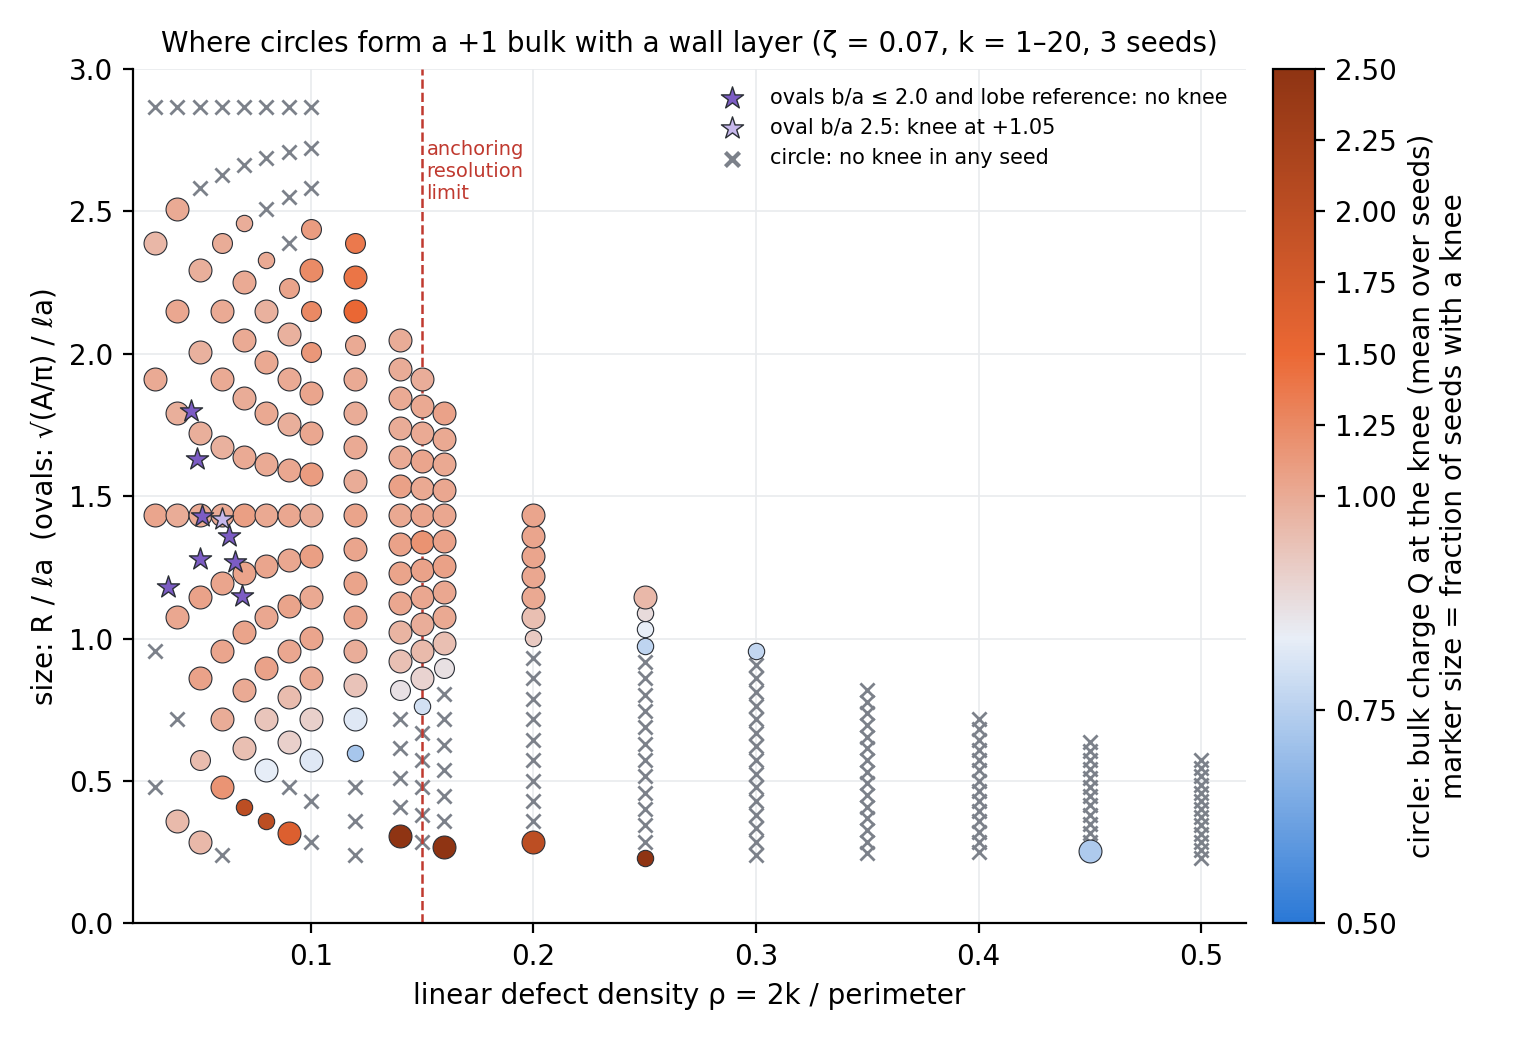
\includegraphics[width=0.85\textwidth]{figs/layer_diagram_circles.png}
\caption{Circles: bulk charge at the knee (colour; marker size = fraction of seeds with a knee; crosses: no knee) in the
plane of linear defect density $\rho=2k/P$ and $R/\la$. Stars: ovals at their own $\rho$ and equivalent radius
$\sqrt{A/\pi}/\la$.}\label{fig:diagram}
\end{figure}
\begin{itemize}
  \item For $\rho\le0.15$, circles form a $+1$ bulk with a pinned wall layer from $R\approx0.75$ to $2.0$--$2.3\,\la$, at all
        densities (knee in 89--100\% of runs, $Q_\mathrm{knee}\approx1.0$, $f_\mathrm{static}\ge0.78$). It degrades above
        $\approx2.5\,\la$ (knee in 15\%) and in very small cavities ($<0.5$--$0.6\,\la$). Beyond the resolution limit
        ($\rho\ge0.2$): mostly no knee.
  \item \textbf{Inscribed-radius test:} circles of $R=0.72$ and $0.96\,\la$ at $\rho\approx0.06$ keep a clean layer
        ($Q_\mathrm{knee}$ 1.03--1.07, $f_\mathrm{static}$ 0.97--0.98). The ovals that lose the layer have inscribed radii
        0.79--1.01\,$\la$ and $\sqrt{A/\pi}$ 1.15--1.8\,$\la$: inside the circle layer region in every size measure
        (Table~\ref{tab:match}). \textbf{The loss is a shape effect.}
  \item The knee finder needed care: the cell-quantised layer produces small steps in $Q(r)$; Q is now smoothed over
        0.045 in $r/R$ before locating the plateau.
\end{itemize}
\begin{table}[h]\centering\small
\caption{Matching ovals with circles (B.~Loewe's point 2): linear density and candidate activity numbers ($/\la$).}\label{tab:match}
\begin{tabular}{lcccccc}\toprule
cavity & $k$ & $\rho=2k/P$ & $\sqrt{A/\pi}$ & half-length & inscribed $r$ & $2A/P$\\\midrule
circle $R=1.43\,\la$ & 6 & 0.060 & 1.43 & 1.43 & 1.43 & 1.43\\
circle $R=1.07\,\la$ & 3 & 0.040 & 1.07 & 1.07 & 1.07 & 1.07\\
oval $b/a=2.5$ (H34) & 6 & 0.060 & 1.42 & 1.53 & 1.30 & 1.41\\
oval $b/a=1.6$ (H34) & 6 & 0.066 & 1.27 & 1.53 & 1.01 & 1.23\\
oval $b/a=1.3$ (H34) & 6 & 0.069 & 1.15 & 1.53 & 0.79 & 1.07\\
oval $b/a=1.6$ (H48) & 6 & 0.046 & 1.80 & 2.16 & 1.43 & 1.74\\
lobe-shaped oval & 3 & 0.036 & 1.18 & 1.37 & 1.00 & 1.16\\\bottomrule
\end{tabular}
\end{table}

\subsection{Mirror runs (H5): the bulk stays positive}
570 runs with winding $-|k|$ (Fig.~\ref{fig:mirror}). $Q(r)$ rises to a \emph{positive} peak before plunging to $-|k|$ at the
wall: the bulk charge is positive, not $-1$, and grows with $|k|$: 0.09 ($|k|=2$), 0.47 (6), 0.83 (10), 1.00--1.02
($|k|=15$--20); the wall carries $\approx2|k|+2\,q_b$ of the $-\frac12$ defects. At fixed size the bulk charge rises with
$|k|$; at fixed $|k|$ it peaks at $R\approx1.5$--$2\,\la$.
\textbf{$+1$ (the Euler characteristic) is the attractor for both winding signs, but activity breaks the mirror symmetry:}
with $+k$ the $+1$ bulk appears at every $k\ge2$ (made of self-propelled $+\frac12$); with $-k$ the wall has to absorb two
extra $-\frac12$, which happens fully only for $|k|\gtrsim13$--15.
\begin{figure}[h]\centering
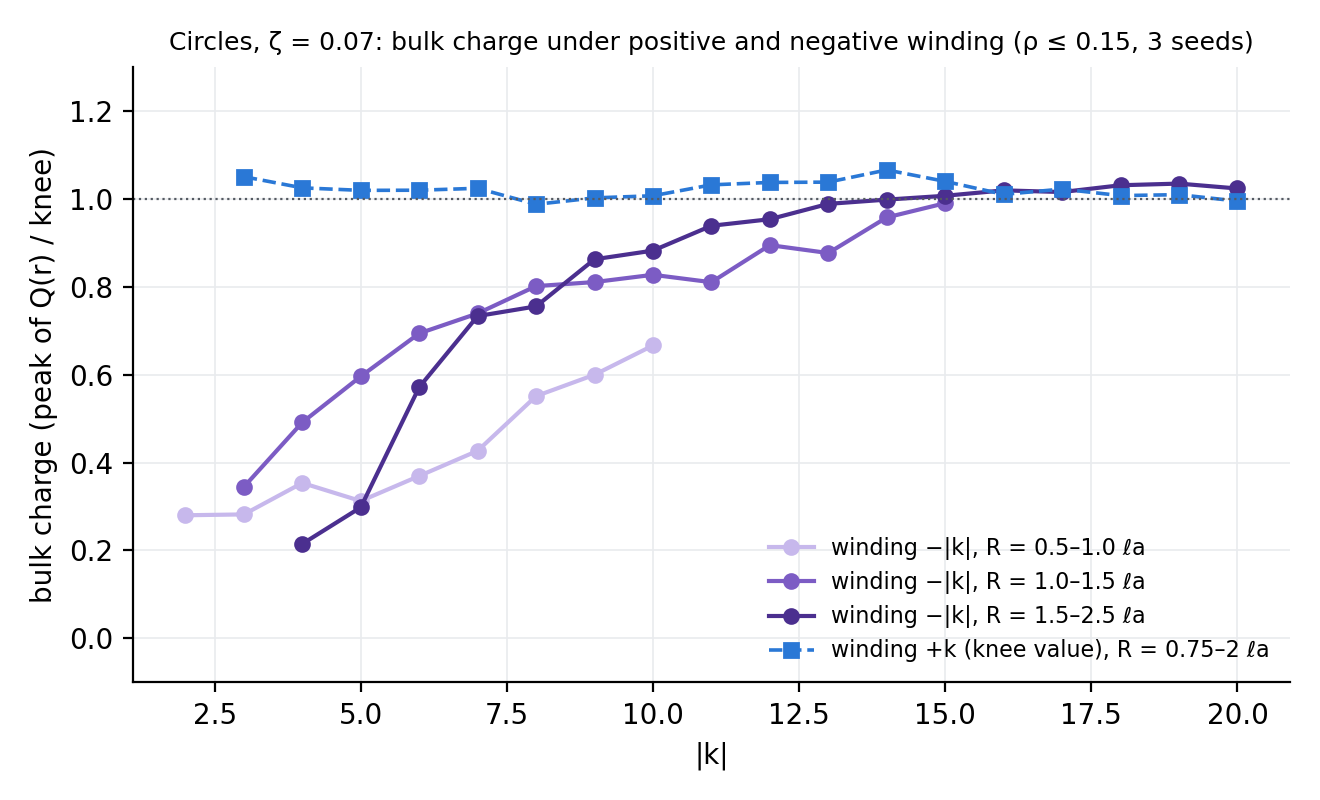
\includegraphics[width=0.8\textwidth]{figs/mirror_bulk_vs_k.png}
\caption{Bulk charge versus $|k|$: positive winding (knee value, squares) and negative winding (peak of $Q(r)$, three size
bins).}\label{fig:mirror}
\end{figure}

\subsection{Shape: size collapse with seeds, and ellipses}
\begin{figure}[h]\centering
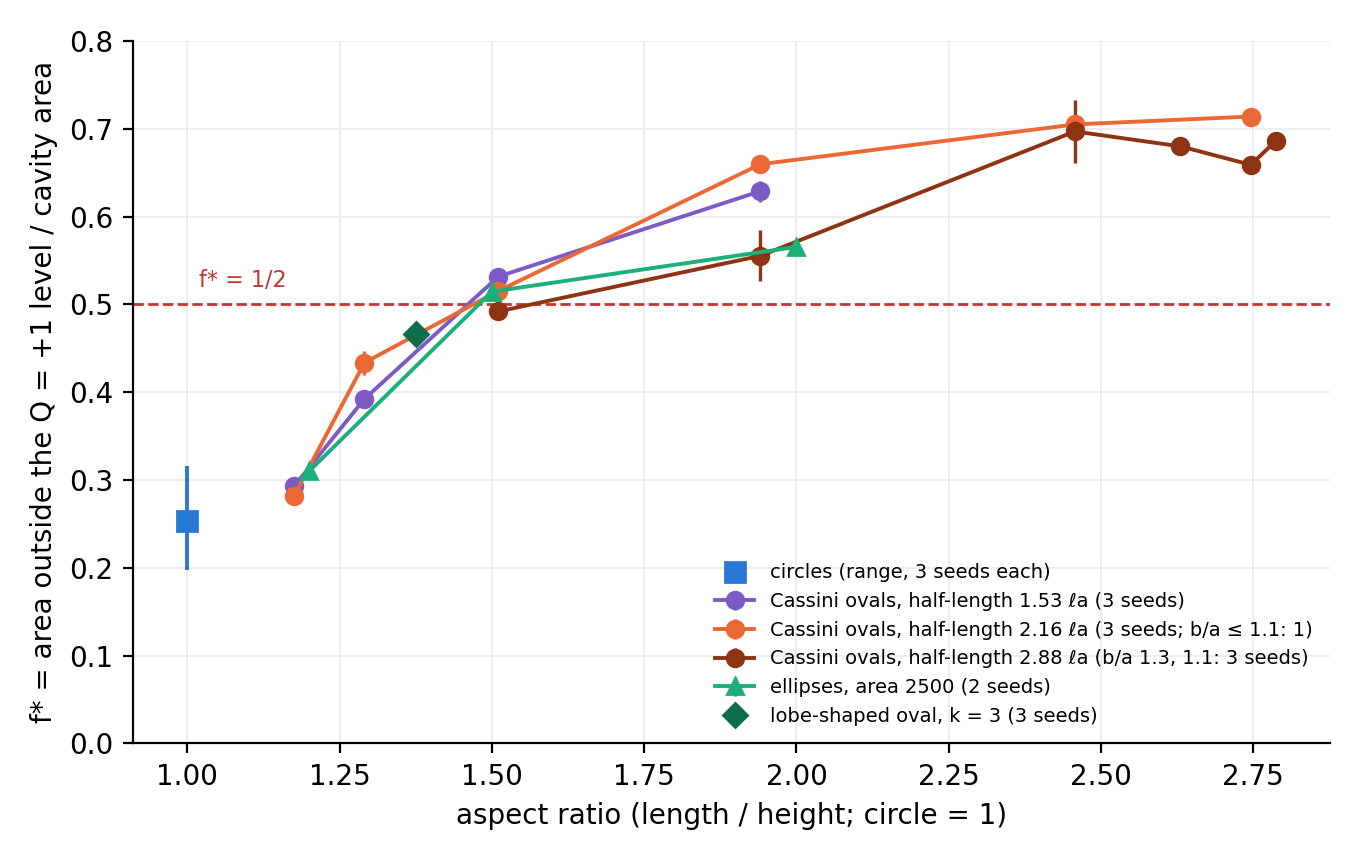
\includegraphics[width=0.85\textwidth]{figs/layer_area_all.png}
\caption{Area fraction outside the $Q=+1$ level versus aspect ratio, all shapes with seeds: Cassini ovals at three sizes,
ellipses (area 2500), the lobe-shaped reference, circles.}\label{fig:areaall}
\end{figure}
\begin{itemize}
  \item \textbf{Size collapse confirmed with seeds:} $f^*$ at half-length 34 / 48 ($1.53$ / $2.16\,\la$): $b/a=2.5$: 0.29 / 0.28;
        2.0: 0.39 / 0.42--0.45; 1.6: 0.53 / 0.49--0.54; 1.3: 0.63 / 0.65--0.67. At $2.88\,\la$ (3 seeds for $b/a$ 1.3, 1.1) slightly
        lower ($\approx0.56$ at aspect 1.94).
  \item \textbf{Ellipses fall on the same curve} (B.~Loewe's question: can a convex cavity lose the layer? \emph{Yes}):
        aspect 1.2: knee 0.98--1.07, $f^*=0.31$, pinned lattice; 1.5: no knee, $f^*=0.51$--0.52; 2.0: no knee, $f^*=0.57$.
        Elongation (aspect $\gtrsim1.4$--1.5) is the generic control for both convex families.
\end{itemize}

\subsection{Dependence on the winding $k$ (B.~Loewe's point 1)}
Half-length 34, $b/a$ 2.0 and 1.6, $k=2\dots12$, 3 seeds. Measured by $Q$ at a fixed depth (no knee needed):
\begin{table}[h]\centering\small
\caption{$Q(c/b=0.85)$ versus $k$ (mean of 3 seeds); knees found (seeds) in brackets.}
\begin{tabular}{lcccccc}\toprule
& $k=2$ & 4 & 6 & 8 & 10 & 12\\\midrule
circle $R=1.43\,\la$ & 0.99 & 0.95 & 0.95 & 0.94 & 0.97 & --\\
oval $b/a=2.0$ & 1.12 & 1.54 & 1.51 & 1.49 & 1.36 & 1.24 (3/3, 1.31)\\
oval $b/a=1.6$ & 1.30 & 2.06 & 1.96 & 1.63 & 1.42 (1/3) & 1.31 (3/3, 1.40)\\\bottomrule
\end{tabular}
\end{table}
The circle is a \emph{traditional} layer ($Q$ at fixed depth independent of $k$). The ovals are neither traditional nor
``all winding into the bulk'': the bulk carries a bounded excess (at most $\approx+1$) at moderate $k$, which shrinks again
as the wall gets crowded; at $k=12$ ($\rho\approx0.13$) a plateau and a wall lattice reappear ($f_\mathrm{static}$ for
$b/a=1.6$: 0.03, 0.21, 0.11, 0.39, 0.70 for $k=2\dots12$). Same trend as the high-$k$ pinched oval and the mirror runs:
\textbf{a crowded wall restores the topological structure}; elongation matters most at moderate imposed density.

\subsection{New layer measures (B.~Loewe's points 1, 3, 4)}
\begin{itemize}
  \item \textbf{Knee of $Q(c)$}: bulk charge from the plateau, no assumption that it is $+1$. Clean circles and the $b/a=2.5$ oval:
        1.0--1.1; elongated ovals and ellipses: no knee. No ``less-charged layer'' (plateau at $+2$, $+3$) in the clean regime;
        large circles at high $k$ ($\rho\approx0.1$--0.12, $R\approx2$--$2.6\,\la$) show a tilted plateau at 1.3--2.1 (to check).
  \item \textbf{Wall Fourier analysis} (density along the wall arclength): instantaneous structure factor $S(m)$, static fraction
        $f_\mathrm{static}=|\langle\rho_m\rangle|^2/\langle|\rho_m|^2\rangle$. Pinned lattice (circles, $b/a=2.5$, ellipse 1.2):
        peak at $m=2k-2$, $S\approx8$--9, $f\approx0.97$--0.99; large circle (2.87\,$\la$): $f=0.87$ (partly sliding);
        elongated ovals and ellipses: $S\approx1.5$--2.7, $f\approx0$--0.4 (no lattice).
  \item \textbf{Heat maps} of the defect positions for all shapes (in the analysis folders).
\end{itemize}

\subsection{Wall--bulk exchange (H7)}
From gap-closed tracks (89--96\% of track ends paired as $\pm\frac12$ events): escape rate of wall $+\frac12$ (per
$10^3$ time units) and mean residence: circles 0.3--0.5 / 900--2000; large circle (2.87\,$\la$) 4.5 / 220; oval $b/a=2.5$
0.7 / 730--970; 2.0: 2.7--3.4 / 200--250; 1.6, 1.3: 5.5--6.2 / 140--150; lobe reference 7.6 / 125. Wall defects in
elongated cavities escape 10--20$\times$ faster; $\le10\%$ of wall visits end in annihilation (the layer empties by undocking).

\subsection{Server}
Sweep complete (1304/1304 on 3 Oct, 0 failures). The \texttt{cassini} branch binary is built and validated on the server
(circle and $a=0$ oval match the production binary). An oval sweep is \textbf{drafted, not launched}
(\texttt{reports/oval\_sweep\_draft.md}): 9 shapes $\times$ 3 equivalent sizes $\times$ 4 densities $\times$ 3 seeds = 324 runs,
$\approx1.2$ days; open choices (mirror subset, high-$\rho$ column, ellipses) listed there.
